\section{Técnicas}

\begin{frame}{Geração de Relevo}
    \begin{itemize}[<+- | alert@+>]
        \item \alert<6>{Ruído de Perlin}
        \item Divisões estocásticas
        \item Falhas geológicas
        \item Deposição de sedimentos
        \item Disposição do ponto médio
    \end{itemize}
\end{frame}

\begin{frame}{Noise}
    Definição:
    \begin{itemize}
        \item Ponto: $Point \in \{ \mathbb{R}^3 \vee \mathbb{R}^2 \vee \mathbb{R}\} $
        \item $ -1 \leq noise(Point) \leq 1$
    \end{itemize}
\end{frame}

\begin{frame}{Noise}
    \begin{figure}
		\centering
        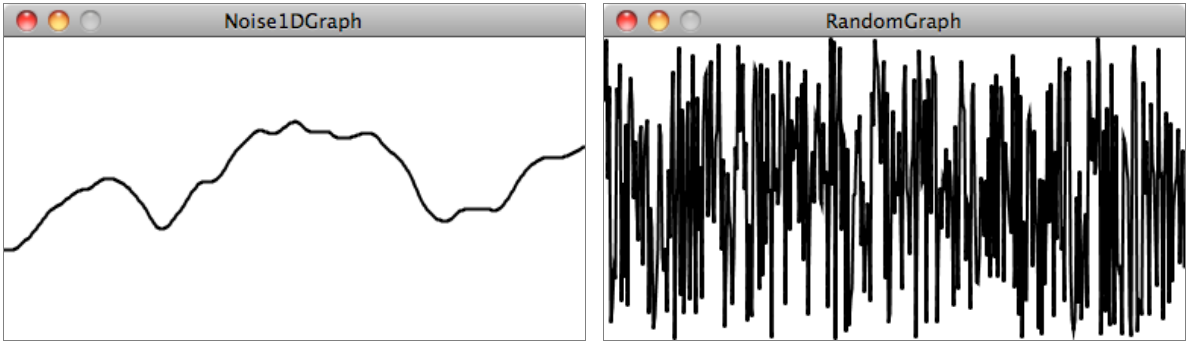
\includegraphics[width=.7\textwidth]{img/explain/noiseRandom.png}
        \caption{\alert{Noise vs Random}, por \cite{shiffman2012nature}.}
    \end{figure}
\end{frame}

\begin{frame}{Noise}
    \begin{figure}
		\centering
        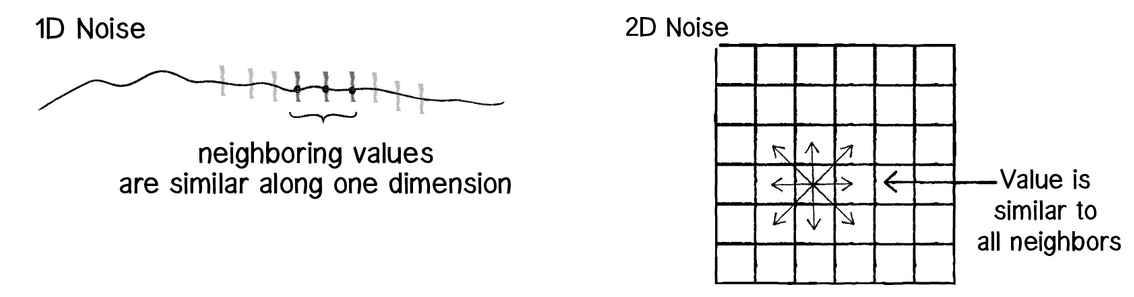
\includegraphics[width=.7\textwidth]{img/explain/1d2dnoise.png}
        \caption{\alert{1d and 2d Noise}, por \cite{shiffman2012nature}.}
    \end{figure}
    \begin{itemize}
        \item Complexidade para $n$ dimensões: $\mathcal{O}(2^n)$
    \end{itemize}
\end{frame}


\begin{frame}{Ruído de Perlin}
    Definição:
    \begin{itemize}
        \item Quantidade de oitavas: $\theta \in \mathbb{N}$
    \end{itemize}
    $$perlinNoise(Point, \theta) = \sum_{t=0}^{t=\theta} \frac{Noise(Point \cdot 2^{t})}{2^{t}}$$
\end{frame}


\begin{frame}{Ruído de Perlin}
    \begin{figure}
		\centering
        \includegraphics[width=.7\textwidth]{img/explain/perlin1d.png}
        \caption{Ruído de Perlin 1D, por \cite{elias2000perlin}.}
    \end{figure}
\end{frame}

\begin{frame}{Ruído de Perlin}
    \begin{figure}
		\centering
        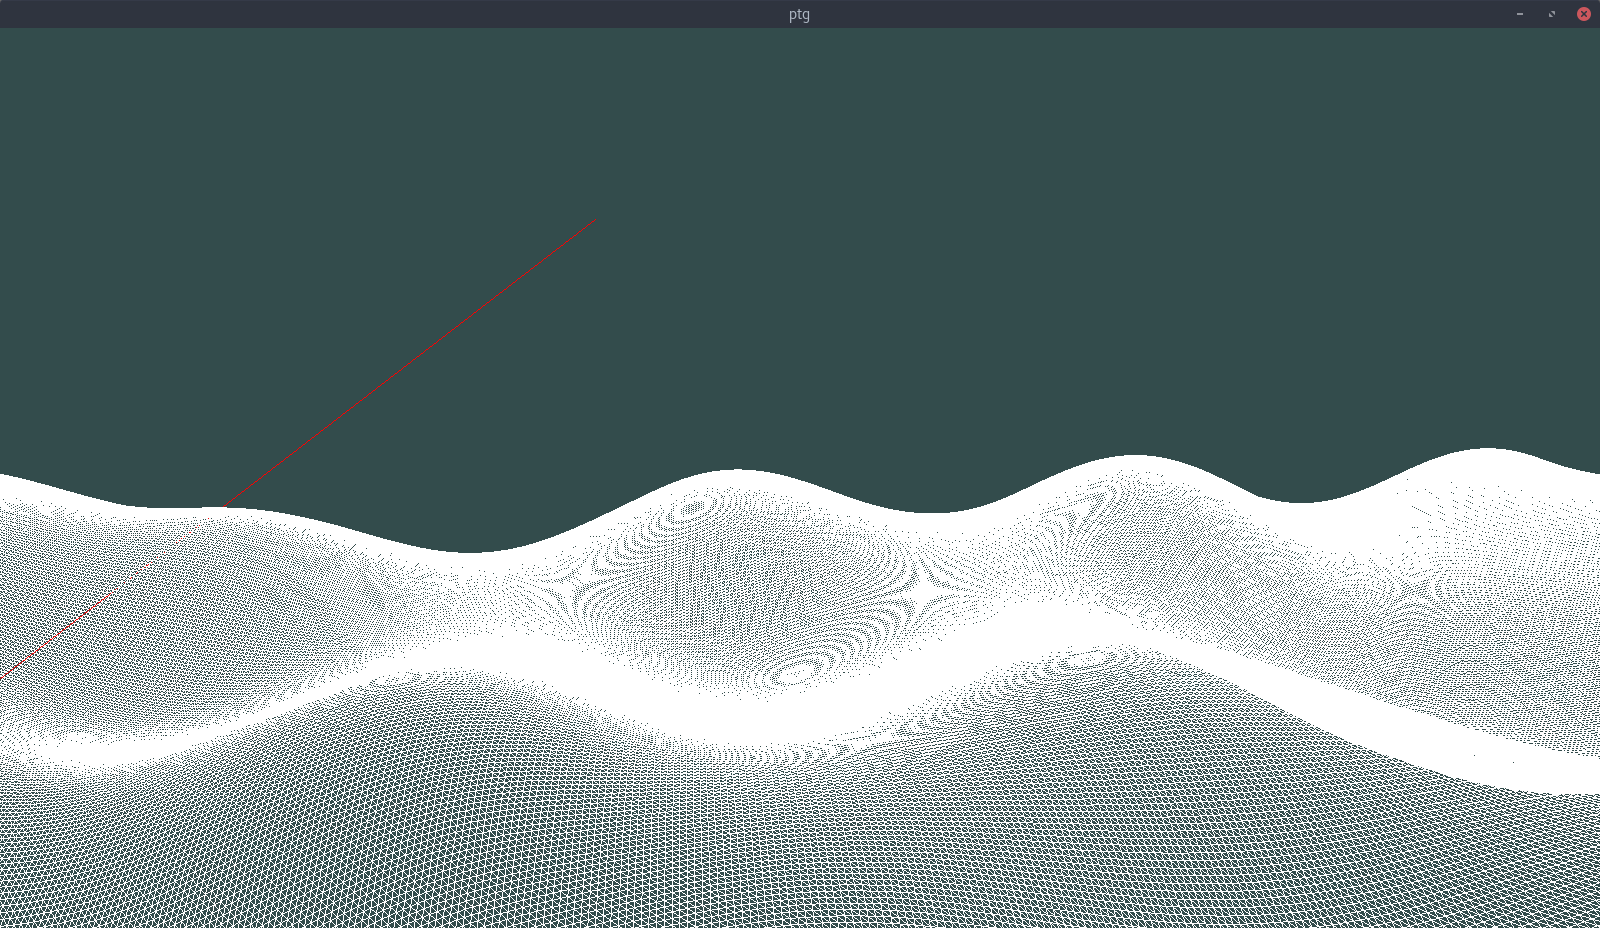
\includegraphics[width=.7\textwidth]{img/explain/octaves1.png}
        \caption{$\theta = 1$.}
    \end{figure}
\end{frame}

\begin{frame}{Ruído de Perlin}
    \begin{figure}
		\centering
        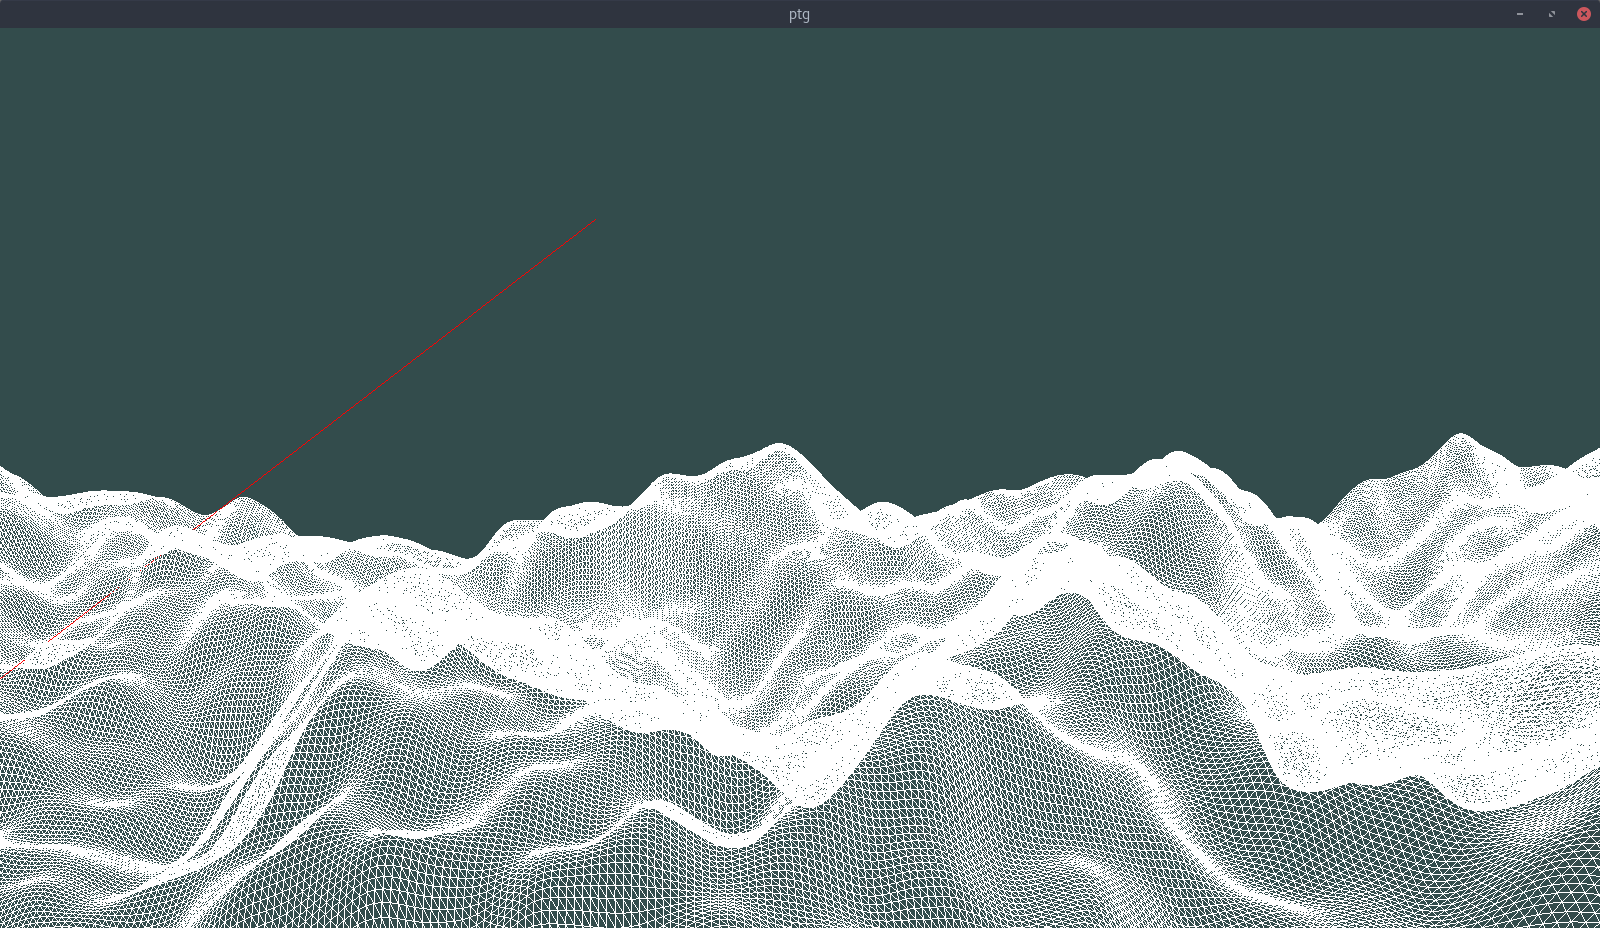
\includegraphics[width=.7\textwidth]{img/explain/octaves4.png}
        \caption{$\theta = 4$.}
    \end{figure}
\end{frame}

\begin{frame}{Ruído de Perlin}
    \begin{figure}
		\centering
        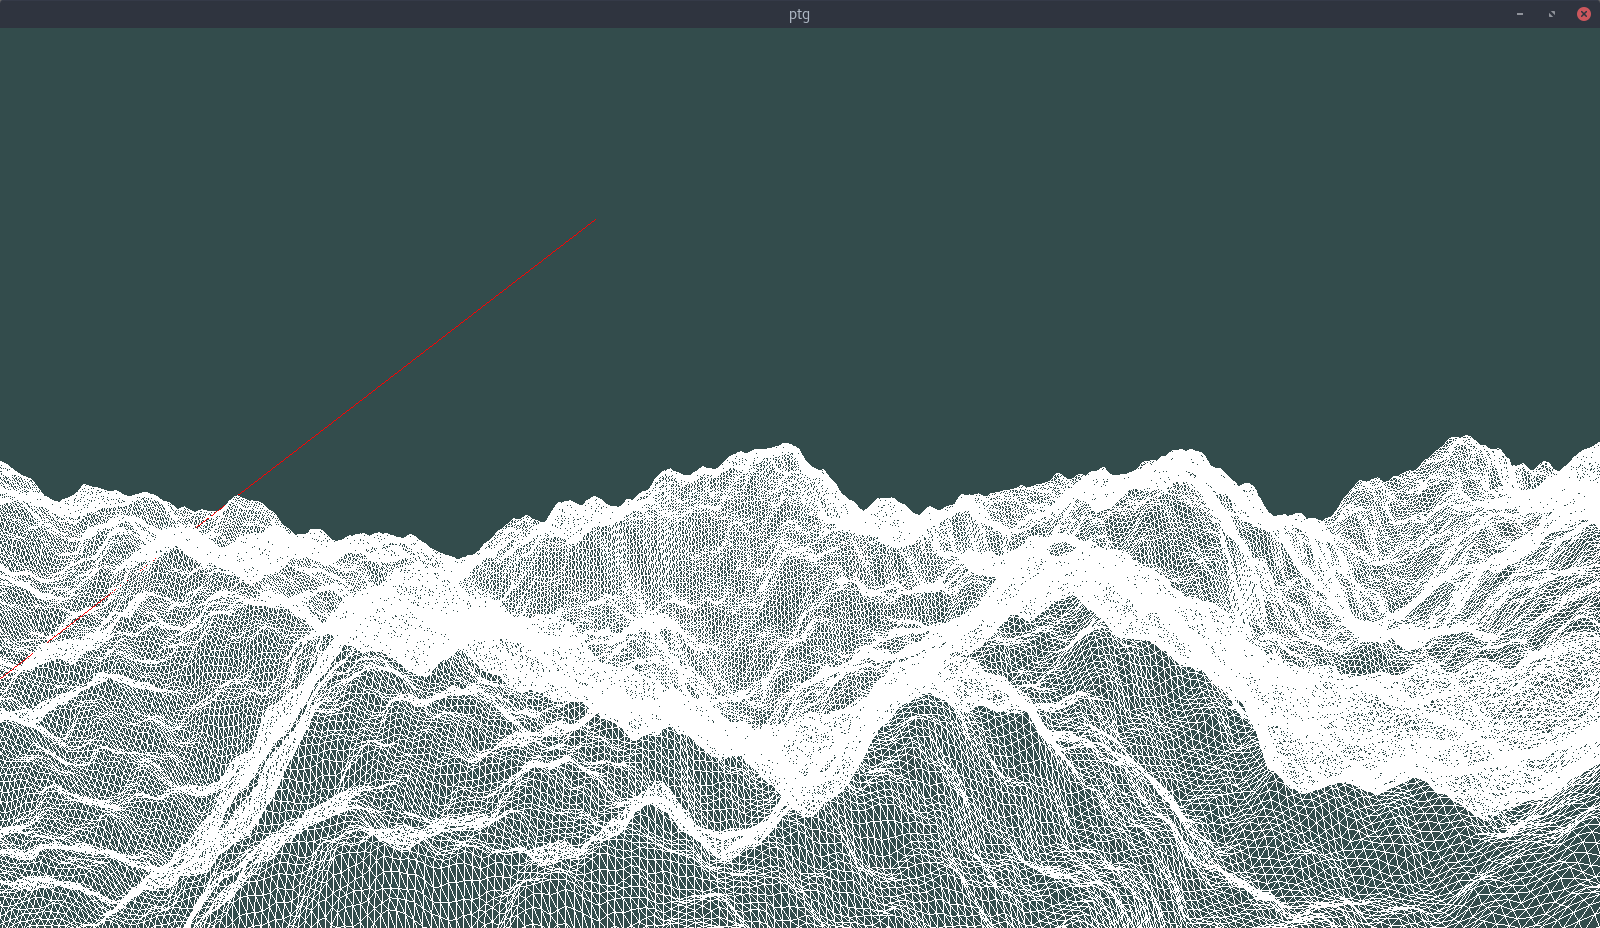
\includegraphics[width=.7\textwidth]{img/explain/octaves16.png}
        \caption{$\theta = 16$.}
    \end{figure}
\end{frame}


% \begin{frame}{Figura Teste}
%   \begin{figure}
% 		\centering
%         \includegraphics[width=.7\textwidth]{img/perlin1d.png}
%         \caption{Ruído de Perlin em uma dimensão.}
%   \end{figure}
% \end{frame}
\begin{frame}{Ruído de Perlin}
    Temos:
    $$\sum_{t=0}^{t=\theta} \frac{Noise(Point \cdot 2^{t})}{2^{t}}$$
    Caso de borda $Noise(Point) = 1$:
    $$\sum_{t=0}^{t=\theta} \frac{1}{2^{t}} = 2^{-\theta} (2^{\theta +1}-1)$$
\end{frame}


\begin{frame}{Ruído de Perlin}
    \begin{equation*}
        \begin{split}
            \visible<+->{max & = \lim_{\theta\to \infty} 2^{-\theta} (2^{\theta +1}-1) \\}
            \visible<+->{& = 2}
        \end{split}
    \end{equation*}
\end{frame}

%mostrar dimenções e manipulações do ruido


%limitações, é realmente infinito?

% Carregar apenas área perto do jogador

% Mostrar o que é tesselation

